\documentclass[10pt]{article}

\usepackage[letterpaper,margin=1in]{geometry}
\usepackage[T1]{fontenc}
\usepackage{hyperref}
\usepackage[parfill]{parskip}
\usepackage{amsmath,amsfonts,amssymb,amsthm}
\usepackage{graphicx}
\usepackage{xcolor}

\graphicspath{{./figs/}}


\vspace{-8ex}
\date{}
\begin{document}

\title{\vspace{-1cm}\textbf{\Large{Intuitive Arm Reach}} \\ \Large{Project Formulation} \\ \textbf{\small{ECE496, 2021-22}}\\\vspace{-0.3cm}}
\author{Defne Dilbaz, Pranshu Malik, Prithvi Marwah, Varun Sampat \\\small{\textbf{Supervisor:}} Professor Mireille Broucke \vspace{-3cm}}

\maketitle

\section{Introduction}
We develop intuition for various tasks through experience. Particularly, we learn to reach for objects in the environment during our infancy, wherein to harness the complexity of our high-dimensional bodies, we are guided by proximodistal patterns of freezing and freeing of degrees of freedom (PDFF), i.e., joints that are closer to the body are more active during self-exploratory movement and more distant joints are progressively involved over the stages of sensorimotor development. This suggests that an innate maturational schedule is involved during sensorimotor development. There is also a related hypothesis, called motor-goal babbling, entailing that we learn to control our bodies by exploring the environment through random movements intended to reach random targets. This way, both hypothetical processes, suggest that through such experiences we develop internal models that allow the movement of limbs in a desired way.

Our project aims to utilize and extend the algorithmic models of aforementioned processes to enable a robotic arm to \emph{intuitively} reach points in its reachable space without the need for explicitly calculating inverse kinematics or dynamics. We heavily rely on the work done in \cite{pdff} which describes how such patterns of exploration can emerge spontaneously as the result of stochastic optimization processes, without explicitly encoding a maturational schedule, and how they can eventually lead to learnt reach actions for a robot. Elements of stochastic optimization also mimic motor babbling and, as a part of the project, we will introduce goal babbling to generate learning data to sample and extend this learning process to the robot's reachable space. To conveniently learn and encode goal-directed movements of the robot, we use a simplified form of dynamical movement primitives (DMPs) \cite{dmps}, which is detailed in appendix \ref{subsec:appendix_terms_def}. Here we formulate the requirements, objectives, and components of the Reach Task Learning Algorithm (RTLA) which will be a result of this project.

\section{Assumptions, Knowns, and Constraints}
The underlying assumption is that the robot, much like an infant, has not yet learned inverse kinematics yet, but the forward kinematics and dynamics models are known for the purpose of simulation and error feedback during learning. Specifically, given a joint configuration $\mathbf{q} \in \mathbb{R}^N$, we are able to calculate the corresponding end-effector position in the world frame, ${^W}\mathbf{p}_{N} = \mathcal{K}(\mathbf{q}) \in \mathbb{R}^p$, through the forward kinematic function for an $N$-DOF robot operating in $p$-dimensional space. There is also no initial reach trajectory involved in the learning process, and thus the algorithm starts from scratch rather than from a demonstration. Since the aim of the algorithm is to learn \emph{how} to reach to a certain position, similar to \cite{pdff}, we disregard the goal-attractor dynamics portion of DMPs, because then there is nothing to learn anymore, i.e., the system will implicitly converge to the goal without the algorithm learning to do that part. Therefore, our control policy is not the full dynamical system with an attractor, but only a radial basis function network (\ref{eqn:dmp_radial_basis}) that generates accelerations in joint space (\ref{eqn:dmp_theta_to_qdd}). Essentially, many assumptions that are standard in conventional robotics, such as goal being the attractor state and warm starts in optimization, are dropped in this developmental science approach to reduce the number of required \emph{auxiliary hypotheses} for understanding and emulating the characteristics of human learning in robots. Initially during the development phase, we will exclusively consider planar robots, i.e., $p=2$, and limit ourselves to robot with spherical wrists, i.e., arm structures for which the end-effector orientation can be decoupled from its position. During simulation run-time or deployment on a physical robot, we will only measure the end-effector and goal positions in the world frame to evaluate the task completion condition, $||{^W\mathbf{p}_{N}} - {^W}\mathbf{p}_{g}|| < R_c$ where $R_c$ is the convergence radius.

\begin{figure}[ht]
\centering
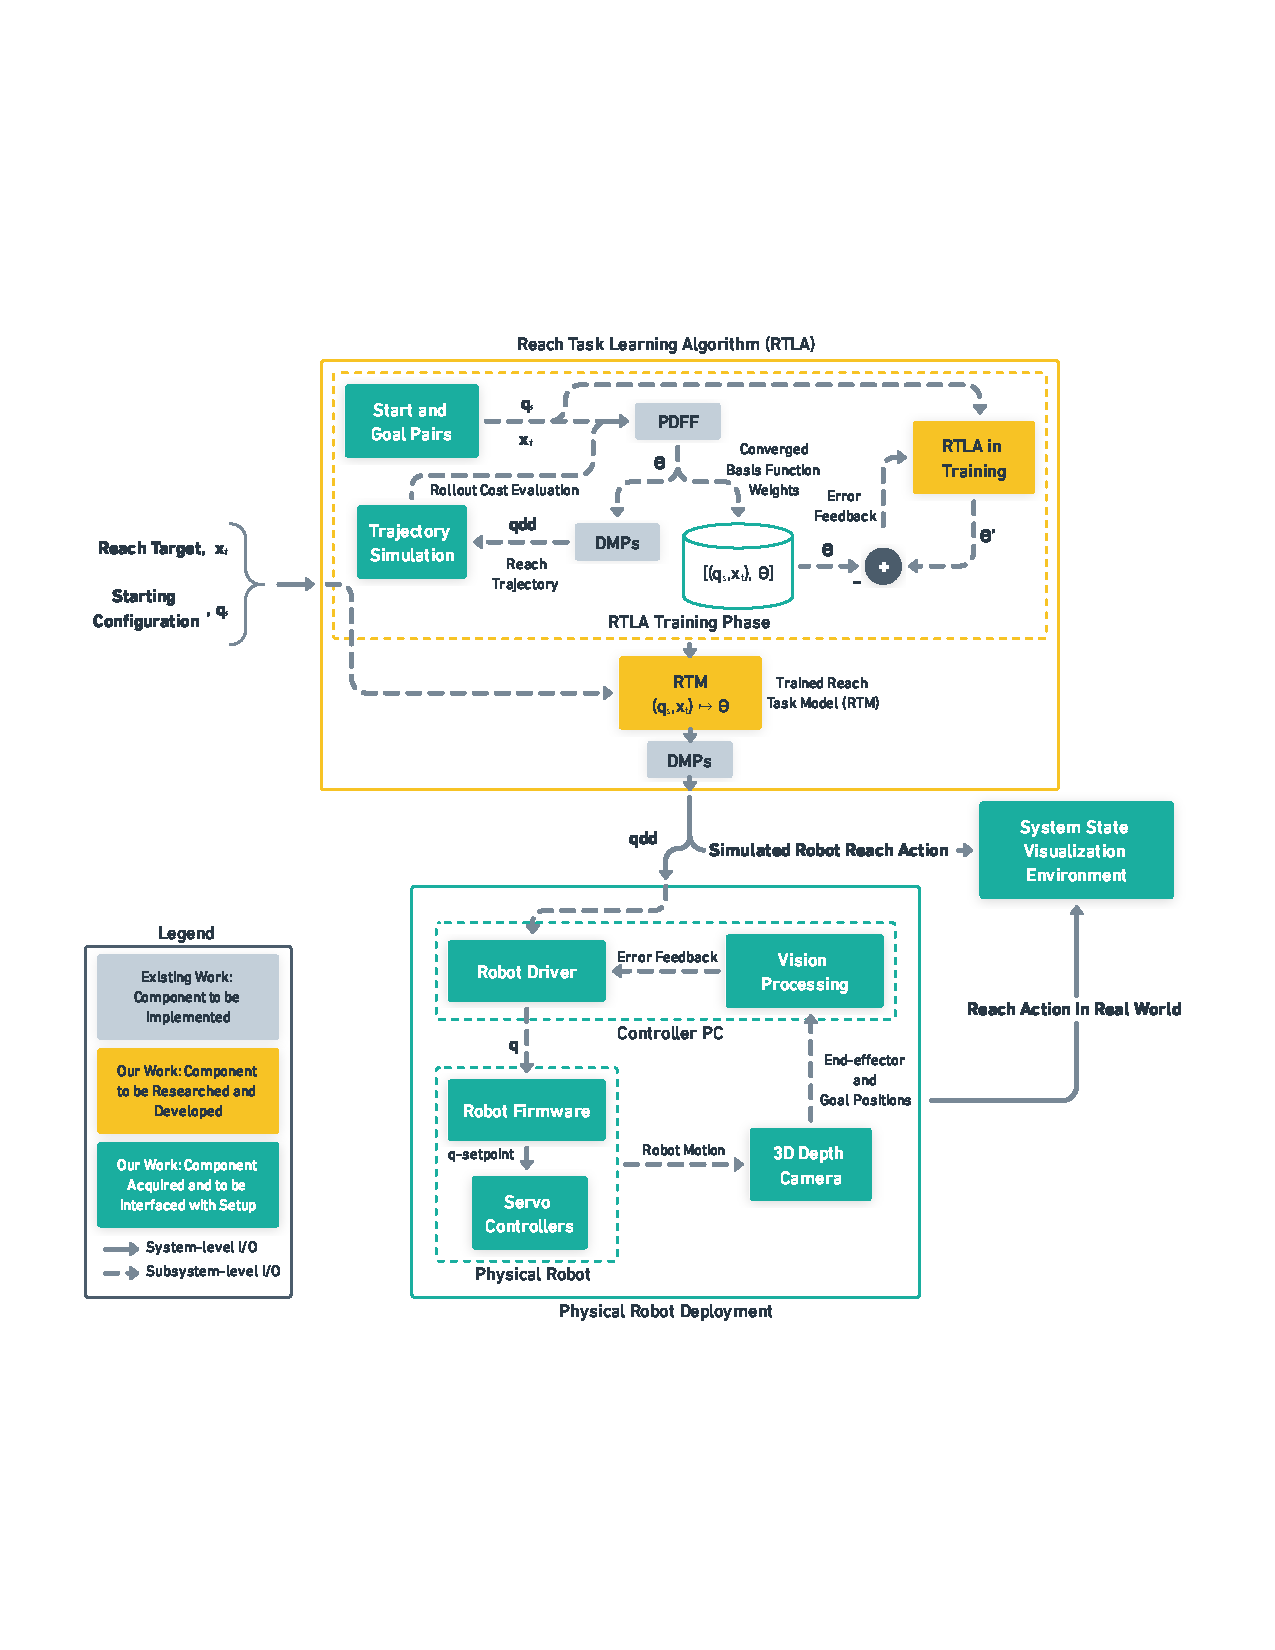
\includegraphics[width=0.7\textwidth]{system_level_overview.pdf}
\label{fig:system_level_overview}
\caption{System level overview}
\end{figure}

\section{Objectives}
We slightly modify the robot arm reach task described above by adding a time-limit $T$ for the reach action, the rationale for which is explained in section \ref{sec:training_algo}. To define the objectives of this task, we borrow the following costs from \cite{pdff} that we would like to minimize together.

\begin{itemize}
	\item \textbf{Reach cost} $||{^W\mathbf{p}_{T, N}} - {^W}\mathbf{p}_{g}||^2$: The squared-distance between the end-effector and the goal positions at the end of the movement ($t = T$). This cost expresses that we want to reach the goal as closely as possible.
	\item\textbf{Comfort cost} $\max(\mathbf{q}_T)$: A cost that corresponds to the largest angle over all  the joints, $0\leq n \leq N$, at the end of the movement. This cost expresses the desire for end-state comfort.
	\item \textbf{Acceleration cost} $r_t$: At each time step $t$, this cost in (\ref{eqn:immediate_cost}) penalizes joint accelerations. The weighting term $(N+1-n)$ penalizes DOFs closer to the origin; the underlying motivation being that wrist movements are less costly than shoulder movements for humans.
\end{itemize}

Thus, we have a terminal cost,

\begin{equation}
\label{eqn:terminal_cost}
	C_T = k_T \cdot \left(||{^W\mathbf{p}_{T, N}} - {^W}\mathbf{p}_{g}||^2 + \max(\mathbf{q}_T)\right)
\end{equation}

and an immediate cost,

\begin{equation}
\label{eqn:immediate_cost}
	r_t  =  k_t \cdot \frac{\sum_{n=1}^N (N+1-n)(\ddot{q}_{t, n})^2}{\sum_{n=1}^N (N+1-n)} \quad .
\end{equation}

Combining, we get the objective function,

\begin{equation}
	\tilde{J}(Q_{\text{dd}}) = C_T\left(\mathcal{K}(\mathbf{q}_T), {^W}\mathbf{p}_{g}, \mathbf{q}_T\right) + \sum_{t=0}^T r_t(\ddot{\mathbf{q}}_t),
\end{equation}

where, $\tilde{J}: \mathbb{R}^{N \times T} \rightarrow \mathbb{R}$ maps the joint accelerations over time, contained in matrix $Q_{\text{dd}}$, to a cost. The overall objective function is $J: \rightarrow \mathbb{R}$, which accepts parameter matrices $\Theta \in \mathbb{R}^{B \times N}$ from the PDFF algorithm and returns corresponding costs. \textcolor{red}{We call this a rollout}. This transformation is described in (\ref{eqn:dmp_theta_to_qdd}). Note that the factors $k_T$ and $k_t$ in (\ref{eqn:terminal_cost}) and (\ref{eqn:immediate_cost}) have the purpose of acting as weights for relative prioritization of objectives and to scale and compensate for different ranges of values for the different cost components. For this project, similar to \cite{pdff}, the order of priorities is: reach close to the goal, achieve end-state comfort, and minimize acceleration.

\section{Inputs}
The inertial world frame $W$, the starting configuration $\mathbf{q}_s \in \mathbb{R}^N$, and the goal position ${^W}\mathbf{p}_{g} \in \mathbb{R}^p$ are the only required inputs for RTLA, or $\mathcal{R}_T$.

\section{Outputs}
Given the above inputs, $\mathcal{R}_T$ will output accelerations in the joint space such that for $\mathbf{q}_T = \int_0^T\int_0^{T}\ddot{\mathbf{q}}(t)\:dt\:dt$ we have $\mathcal{K}(\mathbf{q}_T) \approx {^W}\mathbf{p}_{g}$, ideally for any goal position in the robot's reachable space. The output $\ddot{\mathbf{q}}(t)$ constitutes all the necessary information to carry out the reach action.

\section{Training Algorithm}
\label{sec:training_algo}
PDFF arises during the stochastic optimization. Policy  Improvement with   Black-Box optimization $\text{PI}^{\text{BB}}$
Will use policy improvement through stochastic optimization \cite{pdff} section 3.1.4
Then prescribe what the function approximator RTM is going to do.

\begin{equation}
\label{eqn:dmp_theta_to_qdd}
        \ddot{\mathbf{q}}^\intercal(t) = \mathbf{g}^\intercal(t)\Theta
\end{equation}

Here $\mathbf{g}(t)$ is a vector of $B$ time-dependent normalized radial-basis functions that together describe the joint space trajectory of each joint when scaled by the respective weights. Note that we constrain the number $B$ to be suitable. Too large => extra computation, and hence the time bound $T$. More specifically,

\begin{equation}
\label{eqn:dmp_radial_basis}
    [\mathbf{g}(t)]_b = \frac{\psi_b(t)}{\sum_{b=1}^{B} \psi_b(t)}, \text{ where } \psi_b(t) = \exp{\left(-\frac{(t-c_b)^2}{w^2}\right)}
\end{equation}

Since $\ddot{q}$ is continuous function, we will discretize it into timesteps, $t \in [0, T]$.

Then, we introduce our function approximator, called the Reach Task Model (RTM) that will estimate the parameter matrix theta for a given starting pose and goal location.

\begin{equation}
    \mathcal{R}_M: (\mathbf{q}_s, {^W}\mathbf{p}_{g}) \rightarrow \Theta
\end{equation}

such that ${^W}\mathbf{p}_{T,N} \approx {^W}\mathbf{p}_{g}$. Main thing inside RTLA.

\section{Potential Unique Contributions}
3D robots, first to our knowledge. Also dynamic sims, and RTM. All unique. Also, this has only been implemented in MATLAB, as a first step, that itself will be a meaningful contribution.

\section{Extensions and Future Steps}
Currently posed as an open-loop policy during runtime. Sim-to-real transfer assumed to be perfect. This may be corrected for later by using a full goal-attractor DMP, but the main goal is to evaulate generalization of learning in this new representation. Will be run on real robot and simulation to validate the procedure. Can test for non-sperical wrists, where the should effectively remain the same.

\begin{thebibliography}{5}
\bibitem{pdff}
 Stulp, Freek, and Pierre Yves Oudeyer. 2018. “Proximodistal Exploration in Motor Learning as an Emergent Property of Optimization.” Developmental Science 21 (4): 1–12. DOI: \href{https://doi.org/10.1111/desc.12638}{\texttt{10.1111/desc.12638}}.

\bibitem{dmps}
Jan Ijspeert, Auke, Jun Nakanishi, Heiko Hoffmann, Peter Pastor, and Stefan Schaal. n.d. “Dynamical Movement Primitives: Learning Attractor Models for Motor Behaviors.” Relevant  \href{http://www-clmc.usc.edu/Resources/Software}{\texttt{software}}.
\end{thebibliography}

\pagebreak

\appendix
\section*{Appendices}
\addcontentsline{toc}{section}{Appendices}
\renewcommand{\thesubsection}{\Alph{subsection}}
\subsection{Key Terms and Definitions}\label{subsec:appendix_terms_def}
\subsubsection{Dynamical Movement Primitives (DMPs)}
This is a framework that helps in trajectory planning for dynamical systems to reach a target state. DMPs enable modeling attractor behaviors of autonomous non-linear dynamical systems with the help of statistical learning techniques. It models a simple dynamical system, defined by a set of linear differential equations, and then transforms them into a weakly nonlinear system with prescribed attractor dynamics by means of a learnable autonomous forcing term. Mathematically, this translates to,

\begin{equation}
    \ddot{y} = \alpha_y(\beta_y(y_g-y) - \dot{y}) + f,
\end{equation}

where $\alpha$ and $\beta$ are gain terms, $y$ is the system state, and $y_g$ is the goal state, and $f$ is the non-linear forcing function that helps achieve the goal and generate the trajectory.

The forcing function $f$ is defined as,

\begin{equation}
    f(x,y_g) = \frac{\Sigma_{i = 1}^{N} \psi_i w_i}{\Sigma_{i = 1}^{N} \psi_i}  \cdot x(y_g - y_0),
\end{equation}

where:
\begin{itemize}
	\item $\psi$ is a Gaussian basis function. $\psi_i = e^{-h_i (x - c_i)^2}$
	\item $w_i$ is the weighting given to its corresponding basis function
    \item $x$ is defined as the phase of the system with the dynamics $\dot{x} = - \alpha_x x$. Incorporating $x$ into the forcing function ensures that forcing function diminishes to zero over time. 
	\item $y_g - y_0$ is a spatial scaling term, i.e., scaling the activation of each of these basis functions to be relative to the distance to the target, causing the system to cover more or less distance.
\end{itemize}

Essentially, the forcing function is a set of weighted Guassians, where each Gaussian is located at $c_i$ with variance $h_i$. These Gaussians are activated as the canonical system $x$ converges to its target. 

We will not be using the whole thing, as noted before. We will just learn the f and each joint has its independent transformation system.

\textcolor{red}{x is canonical system?? Check and polish}
\textcolor{red}{Dimension of the DMP??? y state, x state, forcing function. If multidim then how is basis func changed?}

\end{document}